\documentclass{article}
\usepackage{amsmath}
\usepackage{amssymb}
\usepackage{algorithm}
\usepackage{float}
\usepackage{color}
\usepackage{multicol}
\usepackage{forloop}
\usepackage{graphicx}
\usepackage[margin=0.8in]{geometry}
\usepackage{caption}
\usepackage{enumerate}
\usepackage{tikz}
\usepackage{tikz-qtree}
\usepackage{pgfplots}
\usetikzlibrary{%
  arrows,%
  shapes.misc,% wg. rounded rectangle
  shapes.arrows,%
  chains,%
  matrix,%
  positioning,% wg. " of "
  scopes,%
  decorations.pathmorphing,% /pgf/decoration/random steps | erste Graphik
  shadows%
}
\usepackage{tkz-graph}

\graphicspath{ {.} }
\title{MATH 3800 F\\
	\large{Assignment 4}}
\author{Krystian Wojcicki, 101001444}
\date{Winter 2020}

\begin{document}
\maketitle

\begin{enumerate}[1.]

\item \textbf{Consider the following design proposal for a Mars lander module. What is the system
reliability ?}


\tikzset{
  nonterminal/.style={
    % The shape:
    rectangle,
    % The size:
    minimum size=6mm,
    % The border:
    very thick,
    draw=red!50!black!50,         % 50% red and 50% black,
                                  % and that mixed with 50% white
    % The filling:
    top color=white,              % a shading that is white at the top...
    bottom color=red!50!black!20, % and something else at the bottom
    % Font
    font=\itshape
  },
  terminal/.style={
    % The shape:
    rounded rectangle,
    minimum size=6mm,
    % The rest
    very thick,draw=black!50,
    top color=white,bottom color=black!20,
    font=\ttfamily},
  skip loop/.style={to path={-- ++(0,#1) -| (\tikztotarget)}}
}

{
  \tikzset{terminal/.append style={text height=1.5ex,text depth=.25ex}}
  \tikzset{nonterminal/.append style={text height=1.5ex,text depth=.25ex}}
}

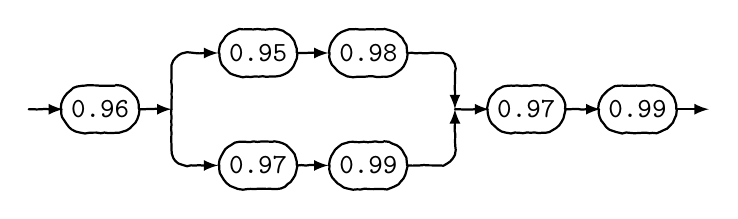
\begin{tikzpicture}[
    >=latex,thick,
    /pgf/every decoration/.style={/tikz/sharp corners},
    fuzzy/.style={decorate,
        decoration={random steps,segment length=0.5mm,amplitude=0.15pt}},
    minimum size=6mm,line join=round,line cap=round,
    terminal/.style={rectangle,draw,fill=white,fuzzy,rounded corners=3mm},
    nonterminal/.style={rectangle,draw,fill=white,fuzzy},
    node distance=4mm
  ]

    \ttfamily
    \begin{scope}[start chain,
            every node/.style={on chain},
            terminal/.append style={join=by {->,shorten >=-1pt,
                fuzzy,decoration={post length=4pt}}},
            nonterminal/.append style={join=by {->,shorten >=-1pt,
                fuzzy,decoration={post length=4pt}}},
%            support/.style={coordinate,join=by fuzzy}
            support/.style={coordinate}
        ]
        \node [support]             (start)        {};
        \node [terminal]                          (E) {0.96};
        \node [support]             (after E)      {};
        \node [support,xshift=7mm]  (between)      {};
        \node [support,xshift=10mm]  (between1)      {};
        \node [support,xshift=7mm]  (before last)  {};
        \node [terminal]                        {0.97};
        \node [terminal]                        {0.99};
        \node [coordinate,join=by ->] (end)        {};
    \end{scope}
    \node (plus)  [terminal,above=of between] {0.95};
    \node (plus1)  [terminal,above=of between1] {0.98};
    \node (minus) [terminal,below=of between] {0.97};
    \node (minus1)  [terminal,below=of between1] {0.99};

    \begin{scope}[->,decoration={post length=4pt},rounded corners=2mm,
            every path/.style=fuzzy]
        \draw (E) -- (after E);
        \draw (after E)     |- (plus);
	\draw (plus) -- (plus1);
        \draw (plus1)        -| (before last);
        \draw (after E)     |- (minus);
	\draw (minus) -- (minus1);
        \draw (minus1)       -| (before last);
    \end{scope}
\end{tikzpicture}

Parallel subsystem: 

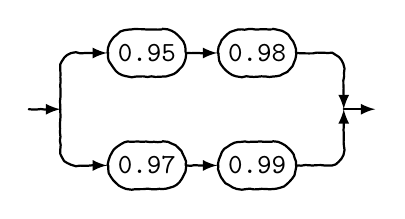
\begin{tikzpicture}[
    >=latex,thick,
    /pgf/every decoration/.style={/tikz/sharp corners},
    fuzzy/.style={decorate,
        decoration={random steps,segment length=0.5mm,amplitude=0.15pt}},
    minimum size=6mm,line join=round,line cap=round,
    terminal/.style={rectangle,draw,fill=white,fuzzy,rounded corners=3mm},
    nonterminal/.style={rectangle,draw,fill=white,fuzzy},
    node distance=4mm
  ]

    \ttfamily
    \begin{scope}[start chain,
            every node/.style={on chain},
            terminal/.append style={join=by {->,shorten >=-1pt,
                fuzzy,decoration={post length=4pt}}},
            nonterminal/.append style={join=by {->,shorten >=-1pt,
                fuzzy,decoration={post length=4pt}}},
%            support/.style={coordinate,join=by fuzzy}
            support/.style={coordinate}
        ]
        \node [support]             (start)        {};
        \node [support]             (after E)      {};
        \node [support,xshift=7mm]  (between)      {};
        \node [support,xshift=10mm]  (between1)      {};
        \node [support,xshift=7mm]  (before last)  {};
        \node [coordinate,join=by ->] (end)        {};
    \end{scope}
    \node (plus)  [terminal,above=of between] {0.95};
    \node (plus1)  [terminal,above=of between1] {0.98};
    \node (minus) [terminal,below=of between] {0.97};
    \node (minus1)  [terminal,below=of between1] {0.99};

    \begin{scope}[->,decoration={post length=4pt},rounded corners=2mm,
            every path/.style=fuzzy]
        \draw (start) -- (after E);
        \draw (after E)     |- (plus);
	\draw (plus) -- (plus1);
        \draw (plus1)        -| (before last);
        \draw (after E)     |- (minus);
	\draw (minus) -- (minus1);
        \draw (minus1)       -| (before last);
    \end{scope}
\end{tikzpicture}

is equivalent to


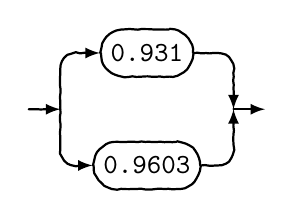
\begin{tikzpicture}[
    >=latex,thick,
    /pgf/every decoration/.style={/tikz/sharp corners},
    fuzzy/.style={decorate,
        decoration={random steps,segment length=0.5mm,amplitude=0.15pt}},
    minimum size=6mm,line join=round,line cap=round,
    terminal/.style={rectangle,draw,fill=white,fuzzy,rounded corners=3mm},
    nonterminal/.style={rectangle,draw,fill=white,fuzzy},
    node distance=4mm
  ]

    \ttfamily
    \begin{scope}[start chain,
            every node/.style={on chain},
            terminal/.append style={join=by {->,shorten >=-1pt,
                fuzzy,decoration={post length=4pt}}},
            nonterminal/.append style={join=by {->,shorten >=-1pt,
                fuzzy,decoration={post length=4pt}}},
%            support/.style={coordinate,join=by fuzzy}
            support/.style={coordinate}
        ]
        \node [support]             (start)        {};
        \node [support]             (after E)      {};
        \node [support,xshift=7mm]  (between)      {};
        \node [support,xshift=7mm]  (before last)  {};
        \node [coordinate,join=by ->] (end)        {};
    \end{scope}
    \node (plus)  [terminal,above=of between] {0.931};
    \node (minus) [terminal,below=of between] {0.9603};

    \begin{scope}[->,decoration={post length=4pt},rounded corners=2mm,
            every path/.style=fuzzy]
        \draw (start) -- (after E);
        \draw (after E)     |- (plus);
        \draw (plus)        -| (before last);
        \draw (after E)     |- (minus);
        \draw (minus)       -| (before last);
    \end{scope}
\end{tikzpicture}

Which is equivalent to 


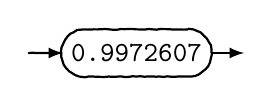
\begin{tikzpicture}[
    >=latex,thick,
    /pgf/every decoration/.style={/tikz/sharp corners},
    fuzzy/.style={decorate,
        decoration={random steps,segment length=0.5mm,amplitude=0.15pt}},
    minimum size=6mm,line join=round,line cap=round,
    terminal/.style={rectangle,draw,fill=white,fuzzy,rounded corners=3mm},
    nonterminal/.style={rectangle,draw,fill=white,fuzzy},
    node distance=4mm
  ]

    \ttfamily
    \begin{scope}[start chain,
            every node/.style={on chain},
            terminal/.append style={join=by {->,shorten >=-1pt,
                fuzzy,decoration={post length=4pt}}},
            nonterminal/.append style={join=by {->,shorten >=-1pt,
                fuzzy,decoration={post length=4pt}}},
%            support/.style={coordinate,join=by fuzzy}
            support/.style={coordinate}
        ]
        \node [support]             (start)        {};
        \node [terminal]                        {0.9972607};
        \node [coordinate,join=by ->] (end)        {};
    \end{scope}

    \begin{scope}[->,decoration={post length=4pt},rounded corners=2mm,
            every path/.style=fuzzy]
    \end{scope}
\end{tikzpicture}

Meaning the entire system can be represented as 

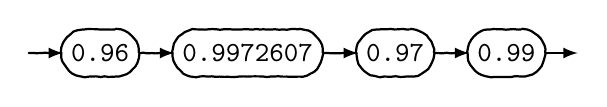
\begin{tikzpicture}[
    >=latex,thick,
    /pgf/every decoration/.style={/tikz/sharp corners},
    fuzzy/.style={decorate,
        decoration={random steps,segment length=0.5mm,amplitude=0.15pt}},
    minimum size=6mm,line join=round,line cap=round,
    terminal/.style={rectangle,draw,fill=white,fuzzy,rounded corners=3mm},
    nonterminal/.style={rectangle,draw,fill=white,fuzzy},
    node distance=4mm
  ]

    \ttfamily
    \begin{scope}[start chain,
            every node/.style={on chain},
            terminal/.append style={join=by {->,shorten >=-1pt,
                fuzzy,decoration={post length=4pt}}},
            nonterminal/.append style={join=by {->,shorten >=-1pt,
                fuzzy,decoration={post length=4pt}}},
%            support/.style={coordinate,join=by fuzzy}
            support/.style={coordinate}
        ]
        \node [support]             (start)        {};
        \node [terminal]                        {0.96};
        \node [terminal]                        {0.9972607};
        \node [terminal]                        {0.97};
        \node [terminal]                        {0.99};
        \node [coordinate,join=by ->] (end)        {};
    \end{scope}

    \begin{scope}[->,decoration={post length=4pt},rounded corners=2mm,
            every path/.style=fuzzy]
    \end{scope}
\end{tikzpicture}

Meaning the entire systems reliability $R_s = (0.96)(0.9972607)(0.97)(0.99)$

\item \textbf{Find the Cholesky decomposition and use it to solve the system of equations.
\begin{gather}
9x + 6y + 12z = 17.4 \\
6x + 13y + 11z = 23.6 \\
12x + 11y + 26z = 30.8
\end{gather}
}

$A = \begin{bmatrix}
9 & 6 & 12 \\
6 & 13 & 11 \\
12 & 11 & 26 \\
\end{bmatrix} , 
b = \begin{bmatrix}
17.4 \\
23.6 \\
30.8
\end{bmatrix} \\
A = GG^T = \begin{bmatrix}
g_{11} & 0 & 0 \\
g_{21} & g_{22} & 0 \\
g_{31} & g_{32} & g_{33} \\
\end{bmatrix}\begin{bmatrix}
g_{11} & g_{21} & g_{31} \\
0 & g_{22} & g_{32} \\
0 & 0 & g_{33} \\
\end{bmatrix} \\ 
g_{11}^2 = 9 \Rightarrow g_{11} = 3 \\
g_{11}g_{21} = 6 \Rightarrow g_{21} = 2 \\
g_{11}g_{31} = 12 \Rightarrow g_{31} = 4 \\
g_{21}^2 + g_{22}^2 = 13 \Rightarrow g_{22} = 3 \\
g_{31}g_{21} + g_{22}g_{32} = 11 \Rightarrow g_{32} = 1 \\
g_{31}^2 + g{32}^2 + g_{33}^2 = 26 \Rightarrow g_{33} = 3 \\$

Therefore
$G = \begin{bmatrix}
3 & 0 & 0 \\
2 & 3 & 0 \\
4 & 1 & 3 \\
\end{bmatrix},
G^T = \begin{bmatrix}
3 & 2 & 4 \\
0 & 3 & 1 \\
0 & 0 & 3 \\
\end{bmatrix}$

$A\bar{x} = b \Rightarrow GG^T\bar{x} = b$ and let $G^T\bar{x} = \bar{y}$ then we have that $G\bar{y} = b$ and $\begin{bmatrix}
3 & 0 & 0 \\
2 & 3 & 0 \\
4 & 1 & 3 \\
\end{bmatrix} \begin{bmatrix}
y_1 \\
y_2 \\ 
y_3 \\
\end{bmatrix} = \begin{bmatrix}
17.4 \\
23.6 \\ 
30.8 \\
\end{bmatrix}$

Meaning $y_1 = 17.4/3 = 5.8, y_2 = (23.6 - 2 * 5.8)/3 = 4, y_3 = (30.8 - 4 * 5.8 - 1 * 4)/3 = 1.2$

Then $G^T\bar{x} = \bar{y} \Rightarrow \begin{bmatrix}
3 & 2 & 4 \\
0 & 3 & 1 \\
0 & 0 & 3 \\
\end{bmatrix}\begin{bmatrix}
x \\
y \\
z \\
\end{bmatrix} = \begin{bmatrix}
5.8 \\
4 \\
1.2 \\
\end{bmatrix}$

So $z = 1.2/3 = 0.4, y = (4 - 0.4)/3 = 1.2, x = (5.8 - 4 * 0.4 - 2 * 1.2)/3 = 0.6$, or $\bar{x} = \begin{bmatrix}
0.6 \\
1.2 \\
0.4 \\
\end{bmatrix}$

Check just to make sure, substitute $\bar{x}$ back into the original set of equations $9(0.6) + 6(1.2) + (12) = 17.4, 6 (0.6) + 13(1.2) + 11(0.4) = 23.6, 12(0.6) + 11(1.2) + 26(0.4) = 30.8$

\item \textbf{Use 5 iterations of Gauss-Seidel to solve the system, starting with x = y = z = 1
\begin{gather}
10x + y + z = 6 \\
x + 10y + z = 6 \\
x + y + 10z = 6
\end{gather}
}

Since the system is already diagonally dominant we can just directly solve for x,y,z.

\begin{center}
\includegraphics{a4_q3}
\end{center}

Check just to make sure, substitute $x=0.5, y = 0.5, z = 0.5$ back into the system. $10 (0.5) + (0.5) + (0.5) = 6, (0.5) + 10(0.5) + (0.5) = 6, (0.5) + (0.5) + 10(0.5) = 6$

\item \textbf{Consider the survival of whales. If the number of whales falls below a minum survival
level m, the species will become extinct. The population is also limited by the carrying
capacity M of the environment.}

\begin{enumerate}[(a)]
\item \textbf{(a) discuss the following model for the whale population $P(t)$ ($k > 0$ is a constant):
$\frac{dp}{dt} = k(M - P)(P - m)$}

Equilibrium when $\frac{dp}{dt} = 0$ which occurs when $P = m$ or $P = M$.

It is easy to see that $\frac{dp}{dt} < 0 $ if $P < m$ or if $P > M$ \\
$\frac{dp}{dt} > 0$ if $m < P < M$.

Therefore if $P < m$ then the population will decline and go to extinction. But if $P > m$ then the population will approach the converging capacity which is $M$.


\item \textbf{(b) graph $dP/dt$ vs $P$ and $P$ vs $t$, considering cases where $P_0 < m, m < P_0 < M$ and
$P_0 > M$}


\usetikzlibrary{intersections}
\begin{tikzpicture}
\begin{axis}[
width=11cm,               
axis lines = middle,  
scaled ticks=false,
no marks,
xmax=20,xmin=0,
ymin=-5,ymax=15,
xlabel=$P$,ylabel=$\frac{dp}{dt}$,
%xtick={-20,...,20},
%ytick={-10,...,10},
yticklabels={,,},
xticklabels={,,},
clip mode=individual
]

\addplot+[name path=A,samples=100, domain=0:20] {(-1)*(x-6)*(x-12)};
\addplot[name path = xaxis,color=black]{0};
\addplot[name path = yaxis,color=black] coordinates {(0,-10) (0,10)};

\node[label={70:{m}},circle,fill,inner sep=2pt] at (axis cs:6,0) {};
\node[label={100:{M}},circle,fill,inner sep=2pt] at (axis cs:12,0) {};

\node[label={70:{max}},circle,fill,inner sep=2pt] at (axis cs:0,9) {};

\node[label={270:{$\frac{m+M}{2}$}},circle,fill,inner sep=2pt] at (axis cs:9,0) {};

\addplot[mark=none, black, ultra thick, dotted] coordinates {(0,9) (9,9)};
\addplot[mark=none, black, ultra thick, dotted] coordinates {(9,0) (9,9)};
\end{axis}
\end{tikzpicture}

$\frac{dp}{dt}$ will reach a max value at $\frac{m + M}{2}$

$\frac{dp}{dt}$ is increasing for $P < \frac{m + M}{2}$ and decreasing when $P > \frac{m + M}{2}$. So $P(t)$ will have an inflection point at $\frac{m + M}{2}$.

\begin{tikzpicture}
\begin{axis}[
width=11cm,               
axis lines = middle,  
scaled ticks=false,
no marks,
xmax=20,xmin=0,
ymin=-5,ymax=15,
xlabel=$t$,ylabel=$P(t)$,
%xtick={-20,...,20},
%ytick={-10,...,10},
yticklabels={,,},
xticklabels={,,},
clip mode=individual
]

\addplot+[name path=A,samples=100, domain=0:20] {      (e^(-0.5 * x)) + 9.05  };
\node[label={180:{$P_0$}},circle,fill,inner sep=2pt] at (axis cs:0,10.05) {};

\addplot+[name path=A,samples=100, domain=0:20] {      (-e^(-0.6 * (x - 0.6))) + 8.95  };
\node[label={180:{$P_0$}},circle,fill,inner sep=2pt] at (axis cs:0,7.517) {};

\addplot+[name path=A,samples=100, domain=0:20] {      (-6)/(1.22 + e^(x-2))   + 8.95  };
\node[label={180:{$P_0$}},circle,fill,inner sep=2pt] at (axis cs:0,4.523) {};

\addplot+[name path=A,samples=100, domain=0:20] {      (-e^(0.3 * x)) + 3  };
\node[label={180:{$P_0$}},circle,fill,inner sep=2pt] at (axis cs:0,2) {};

\addplot[name path = xaxis,color=black]{0};
\addplot[name path = yaxis,color=black] coordinates {(0,-10) (0,10)};

\addplot[mark=none, black, thick, dotted] coordinates {(0,9) (20,9)};
\node[label={180:{M}},circle,fill,inner sep=2pt] at (axis cs:0,9) {};

\addplot[mark=none, black, thick, dotted] coordinates {(0,6) (20,6)};
\node[label={180:{$\frac{m+M}{2}$}},circle,fill,inner sep=2pt] at (axis cs:0,6) {};

\addplot[mark=none, black, thick, dotted] coordinates {(0,3) (20,3)};
\node[label={180:{m}},circle,fill,inner sep=2pt] at (axis cs:0,3) {};


\end{axis}
\end{tikzpicture}

The blue line shows $P$ is decreasing and concave up. The horizontal line at $M$ shows the carrying capacity and an equilibrium solution. The red line shows $P$ is increasing and concave down, the entire portion between $M$ and $\frac{m + M}{2}$ is concave down.. The horizontal line at $\frac{m+M}{2}$ shows the inflection point. The brown line shows $P$ is increasing and concave up (between the third $P_0$ and $\frac{m + M}{2}$). The horizontal line at $m$ shows minimum survival level and an equilibrium solution. Below that the black line shows P is decreasing and concave down.

\item \textbf{(c) solve the model and show that $P(t) \Rightarrow M$ as $t \Rightarrow \infty$ (provided what ?)}

$\frac{dp}{dt} = k(M - P)(P - m) = \frac{dp}{(M - P)(P - m)} = kdt$

Partial Fractions gives us $\frac{1}{(M-P)(P-m)} = \frac{a}{M-P} + \frac{b}{P - m} \Rightarrow a = b = \frac{1}{M - m}$

Meaning we have $(\frac{1}{M-P} + \frac{1}{P - m})dp = k(M - m)dt$

Integrate on both sides $\int(\frac{1}{M - P} + \frac{1}{P - m})dp = \int{k(M - m)dt}$\\
$-ln|M - P| + ln|P - m| = k(M - m)t + C$

Take to $e^x$, $\frac{P - m}{M - P} = Ke^{k(M - m)t}$

Solving for $P$ we get $P(t) = \frac{m + MKe^{k(M-m)t}}{1 + Ke^{k(M-m)t}}$

$\lim_{t \to \infty} P(t) = \lim_{t \to \infty} \frac{m + MKe^{k(M-m)t}}{1 + Ke^{k(M-m)t}}, \text{ using L'hopital's rule } \Rightarrow \lim_{t \to \infty} \frac{MKe^{k(M-m)t}}{Ke^{k(M-m)t}} = M$ Provided that $P_0 > m$. 

\item \textbf{(d) discuss how you would test the model and how you would determine $m$ and $M$}

We could estimate $M$ from a plot of data and estimate $\frac{m + M}{2}$ by looking for the change in concavity and the maximum growth location. We could then estimate for $m$ utilizing $M$. Then if we plot $ln\frac{P - m}{M - P}$ versus $t$ we should have a linear function which we can use to test the model. If the population falls below m, the population will go to zero rapidly. So care must be taken to ensure $P > m$ at all times. 

\end{enumerate}

\end{enumerate}
\end{document}